%%%%%%%%%%%%%%%%%%%%%%%%%%%%%%%%%%%%%%%%%
% Beamer Presentation
% LaTeX Template
% Version 1.0 (10/11/12)
%
% This template has been downloaded from:
% http://www.LaTeXTemplates.com
%
% License:
% CC BY-NC-SA 3.0 (http://creativecommons.org/licenses/by-nc-sa/3.0/)
%
%%%%%%%%%%%%%%%%%%%%%%%%%%%%%%%%%%%%%%%%%

%----------------------------------------------------------------------------------------
%	PACKAGES AND THEMES
%----------------------------------------------------------------------------------------

%\documentclass{beamer}
\documentclass[aspectratio=169]{beamer}

\usepackage[utf8x]{inputenc}
\usepackage{url}
\usepackage{eqnarray}
\usepackage{graphicx}
%\usepackage[spanish]{babel}
\usepackage{mathtools}
\usepackage{color}
\DeclarePairedDelimiter{\ceil}{\lceil}{\rceil}

\mode<presentation> {

% The Beamer class comes with a number of default slide themes
% which change the colors and layouts of slides. Below this is a list
% of all the themes, uncomment each in turn to see what they look like.

%\usetheme{default}
%\usetheme{AnnArbor}
%\usetheme{Antibes}
%\usetheme{Bergen}
%\usetheme{Berkeley}
%\usetheme{Berlin}
%\usetheme{Boadilla}
%\usetheme{CambridgeUS}
%\usetheme{Copenhagen}
%\usetheme{Darmstadt}
%\usetheme{Dresden}
%\usetheme{Frankfurt}
%\usetheme{Goettingen}
%\usetheme{Hannover}
%\usetheme{Ilmenau}
%\usetheme{JuanLesPins}
%\usetheme{Luebeck}
%\usetheme{Madrid}
%\usetheme{Malmoe}
%\usetheme{Marburg}
%\usetheme{Montpellier}
%\usetheme{PaloAlto}
%\usetheme{Pittsburgh}
%\usetheme{Rochester}
%\usetheme{Singapore}
%\usetheme{Szeged}
\usetheme{Warsaw}
\usecolortheme[rgb={0.8,0.0,0.26}]{structure}

% As well as themes, the Beamer class has a number of color themes
% for any slide theme. Uncomment each of these in turn to see how it
% changes the colors of your current slide theme.

%\usecolortheme{albatross}
%\usecolortheme{beaver}
%\usecolortheme{beetle}
%\usecolortheme{crane}
%\usecolortheme{dolphin}
%\usecolortheme{dove}
%\usecolortheme{fly}
%\usecolortheme{lily}
%\usecolortheme{orchid}
%\usecolortheme{rose}
%\usecolortheme{seagull}
%\usecolortheme{seahorse}
%\usecolortheme{whale}
%\usecolortheme{wolverine}

%\setbeamertemplate{footline} % To remove the footer line in all slides uncomment this line
%\setbeamertemplate{footline}[page number] % To replace the footer line in all slides with a simple slide count uncomment this line

%\setbeamertemplate{navigation symbols}{} % To remove the navigation symbols from the bottom of all slides uncomment this line
}
%\newcommand{\abrcuatrimetre}{sep_dic_2020}
\usepackage{graphicx} % Allows including images
\usepackage{booktabs} % Allows the use of \toprule, \midrule and \bottomrule in tables

%----------------------------------------------------------------------------------------
%	TITLE PAGE
%----------------------------------------------------------------------------------------
\newcommand{\nombreMateria}{Fundamentos de Sistemas de Informaci\'on}
\newcommand{\programaAcademico}{Maestr\'ia en Ingenier\'ia}
\newcommand{\cuatrimestre}{Agosto -- Diciembre 2024}
\newcommand{\abreviaturaNombreMateria}{MI}
\newcommand{\claveClassroom}{siudfqm}
\newcommand{\claveMeet}{https://meet.google.com/gxn-insx-bbf}
\title{\nombreMateria} % The short title appears at the bottom of every slide, the full title is only on the title page

\author{Dr. Marco Aurelio Nuño Maganda} % Your name
\institute[UPV] % Your institution as it will appear on the bottom of every slide, may be shorthand to save space
{
Universidad Politecnica de Victoria \\ % Your institution for the title page
\programaAcademico \\ % Your institution for the title page
\cuatrimestre  \\ % Your institution for the title page
\medskip
\textit{mnunom@upv.edu.mx} % Your email address
}
\date{\today} % Date, can be changed to a custom date

\addtobeamertemplate{navigation symbols}{}{%
    \usebeamerfont{footline}%
    \usebeamercolor[fg]{footline}%
    \hspace{1em}%
    %\insertframenumber/\inserttotalframenumber
    \insertframenumber
}
\usepackage{setspace}

\usepackage[spanish]{babel}

\begin{document}

\begin{frame}
\titlepage % Print the title page as the first slide
\end{frame}




%------------------------------------------------
\section{Presentación} 

\begin{frame}

\frametitle{Breve CV del Facilitador}
\begin{itemize}
\item Doctor en Ciencias Computacionales por parte del INAOE (2009).  
\item Profesor de Tiempo Completo de la UPV desde 2009.  
\item Miembro del Sistema Nacional de Investigadores - Nivel Candidado (2014-2016), Nivel I (2020-2022), Nivel I (2023-2027)
\item 17 tesis dirigidas a nivel maestría.
\item Asignaturas impartidas en el pasado 
\begin{itemize}
\item Licenciatura: Cómputo en Dispositivos Moviles, Graficación por Computadora Avanzada, Lenguajes y Automátas, Programación Orientada a Objetos
\item Maestr\'ia: Visi\'on por computadora, T\'opicos Selectos de Imagenolog\'ia, Fundamentos de Sistemas de Informaci\'on
\end{itemize}
\item Miembro del N\'ucleo Acad\'emico B\'asico (NAB) de la maestria en Ingeniería de la UPV.
\end{itemize}
\end{frame}


\section{Horario de Clase}

\begin{frame}
\begin{itemize}
\frametitle{Plataforma Virtual para el Curso}
\item Nombre de la clase: \textbf{\nombreMateria-\cuatrimestre}
\item Código de clase en Classroom: \textbf{\claveClassroom}
\item Enlace Meet para sesiones no presenciales: \textbf{\claveMeet}
\end{itemize}
\end{frame}

\begin{frame}
\frametitle{Horario de la Clase}


\begin{itemize}
\item Días y horas de clase
\tiny
\begin{spacing}{1.0}
\begin{center}
\begin{tabular}{c|ccccc}
\hline 
\textbf{Clave de Grupo}          & Lunes           & Martes       & Miércoles      & Jueves          & Viernes        \\  \hline 
%IM-20333  & 12:05 - 13:55   &              & 12:05 - 13:55  &                 &                \\
IM-20375  & 12:05 - 13:55   &              & 12:05 - 13:55  &                 &                \\
%ITI-271093 & 14:54-15:50 & 13:00-13:55  & 14:55-15:50 &  14:00 - 15:50  & 14:54-15:50    \\      
\hline
\end{tabular}
\end{center}
\end{spacing}
\normalsize
\item Fechas Importantes:
\begin{itemize}
\item Inicio de Cursos: 4/Septiembre
\item Fin de Cursos: 12/Diciembre
\item Dias no hábiles oficiales: 20 de noviembre (lunes). 
\end{itemize}
\end{itemize}

\end{frame}






\begin{frame}
\frametitle{Reglas básicas}
\begin{itemize}
\item Se recomienda puntualidad y asistencia a las sesiones.
\item Respecto hacia el profesor y hacia sus compañeros y compañeras.  
\item No se permite el ingreso y/o ingestión de \textbf{Alimentos} ni \textbf{Bebidas}. 
%\item \textbf{NO SE PERMITE EL USO de AUDIFONOS O DISPOSITIVOS MANO-LIBRES EN CLASE. De detectar esta situaci\'on, se amonestar\'a al estudiante y de reiterar, dicho estudiante ser\'a expulsado de CURSO por el resto del CUATRIMESTRe, sin derecho a r\'eplica. }
%Cámaras deben encenderse en el momento que se les solicite, además de estar a la vista. 
\end{itemize}
\end{frame}

\begin{frame}
\frametitle{Pase de Lista}
\begin{itemize}
\item Pase de Lista al Inicio de cada sesi\'on.
\item Para actividades en linea, debe utilizar su cuenta institucional de la universidad, ya que no se autorizará el ingreso de ningún participante externo a la universidad.  
\item Para justificar una inasistencia, es necesario cumplir con los siguientes pasos:
\begin{itemize}	 
\item Mandar correo al profesor, justificando su inasistencia (solo por motivos m\'edicos)
\end{itemize}
\end{itemize}
\end{frame}


\begin{frame}
\frametitle{Asistencias m\'inimas para aprobar asignatura}
\begin{itemize}
\item Es obligatorio tener un 90\% de asistencia. De no ser as\'i, el estudiante PIERDE su derecho de ser EVALUADO
\end{itemize}
\begin{block}{Alumnos VIPs}
En caso de tener un empleo formal dentro o fuera de la ciudad, es necesario entregar una \textbf{constancia laboral} que acredite el horario que se esta cubriendo (en el caso de locales, este horario se debe empalmar con el de la materia). En esa constancia debe acreditar que se esta haciendo labores de manera presencial en tal ubicacion. Esto lo dispensa solo del requisito de las asistencias, mas no de los proyectos que deban entregarse. Incluso pudiera solicitarle presentar avance de manera ``remota'' durante alguna de las clases. Enviar esa constancia con copia para el director de carrera.
\end{block}
\end{frame}





\begin{frame}
\frametitle{Justificaci\'on de Faltas Extraordinaria}
\begin{itemize}
\item Todo aquel estudiante que realice una estancia de investigaci\'on, visita acad\'emica, visita a empresa, evento deportivo (por parte de la Universidad), o cualquier otra actividad acad\'emica, debe negociar una extesi\'on m\'axima de \textbf{7 d\'ias naturales} de pr\'orroga para entrega de proyectos individuales, en equipo o asignaciones especiales, respaldado por algun documento oficial que acredite dicha actividad. 
\item Ninguna actividad de las anteriormente mencionadas \textbf{es causa de EXENSI\'ON} de los proyectos solicitados en la clase, ni generar\'a ning\'un cambio o ajuste a sus calificaciones por participar en dicho evento.  De no cumplir con los plazos de entrega establecidos, deber\'a asumir las consecuencian de no entregar los proyectos o trabajo solicitado en el tiempo establecido.
\item Las inasistencias a clase quedan justificadas solo \textbf{durante el desarrollo del evento y los translados}. Para justificar dichas inasistencias, debe hacerlo mediante el procedimiento establecido para dicha justificaci\'on.

\end{itemize}

\end{frame}




%
\begin{frame}
\section{Temas a cubrir}
\frametitle{Unidades }
\begin{enumerate}

\item Introducción a la Inteligencia Artificial
\begin{enumerate}
\item Inteligencia Artificial y Sistemas Inteligentes
\item Razonamiento y representación del conocimiento
\item Estrategias de Búsqueda
\end{enumerate}

\item Técnicas Básicas de Aprendizaje
\begin{enumerate}
\item Aprendizaje Supervisado y No Supervisado
\item Aprendizaje basado en Redes Neuronales
\item Algoritmos Genéticos
\end{enumerate}

\item Introducción a la percepción automática
\begin{enumerate}
\item Percepción Visual
\item Percepción Visual Estereoscópica
\item Procesamiento de Lenguaje Natural
\end{enumerate}

\end{enumerate}

\end{frame}

\begin{frame}
\section{Temas a cubrir}
\frametitle{Temas a cubrir }
\begin{enumerate}

\item Introducción a las tecnolog\'ias de la informaci\'on
\item Herramientas para escritura de documentos cient\'ificos
\item Programaci\'on orientada a objetos e interfaces de usuario
\item Programaci\'on en dispositivos m\'oviles
\item T\'opicos avanzados
\end{enumerate}

\end{frame}


%------------------------------------------------
\section{Evaluación}
%------------------------------------------------

\begin{frame}
\frametitle{Evaluación (1)}
Para cada unidad del curso, se consideran los siguientes aspectos:
\begin{itemize}
\item Exposicion de Tema Selecto 1- 10\%
\item Exposicion de Tema Selecto 2- 10\%
\item Proyecto Individual 1 - 20\%
\item Proyecto Individual 2 - 20\%
\item Proyecto Individual 3 - 20\%
\item Proyecto Individual 4 - 20\%
\end{itemize}
Para aprobar el curso, es obligatorio entregar todos los proyectos solicitados
%Para tener derecho a una evaluacion de recuperacion de la unidad, el estudiante debe haber cumplido con 2 /3 requisitos de la unidad, y esta recuperación aplica solamente UNA VEZ a lo largo del cuatrimestre.
\end{frame}

\begin{frame}
\frametitle{Evaluación (2)}
Para cada unidad, habra sesiones de ``teoria'', sesiones de seguimiento de proyectos y sesiones de esparcimiento
\begin{itemize}
\item En las sesiones de teoria, el profesor presentara uno o varios temas
\item En las sesiones de seguimiento de proyectos, de manera aleatoria se nombrara al integrante de equipo individual o en equipo. En el caso de que un integrante individual no responda, se le bajarán 5 puntos a su calificación del proyecto
\item En las sesiones de esparcimiento, se permitirá a los estudiantes trabajar en proyectos pendientes, pero se contabilizará la asistencia. 
\end{itemize}
\end{frame}

\begin{frame}
\frametitle{Evaluación (3)}
Sesiones de Seguimento de proyectos
\begin{itemize}
\item Programadas generalmente una semana despues de haber sido asignado el proyecto
\item Los estudiantes deben exponer el avance del proyecto, as\'i como los retos y dificultades sorteados
%\item En el caso de que el integrante del equipo seleccionado aleatoriamente no responda satisfactoriamente lo cuestionado, se le bajaran 5 puntos a su calificacion del proyecto a todos los integrantes del equipo
%\item En el caso de los proyectos en equipo, el integrante seleccionado es aleatorio. Si en una primera ronda le toco al integrante A, en una segunda ronda posiblemente le toque al integrante B
\end{itemize}
\end{frame}


\begin{frame}
\frametitle{Evaluación (4)}
Acerca de los proyectos
\begin{itemize}
\item Proyectos diferentes para los integrantes de la clase 
\item Asignados de manera aleatoria para cada integrante de la clase
\end{itemize}
\end{frame}




%
\begin{frame}
\frametitle{Cartucho de Recuperación (REC)}
\begin{itemize}
\item Estudiante tiene derecho a solicitar un ÚNICO proyecto de recuperación aplicable a un solo proyecto o actividad.
\item Esta solicitud debe HACERLA es estudiante - El profesor NO ES RESPONSABLE de informar al estudiante cuando tiene un ADEUDO.  
\item Si el proyecto no entregado es individual, se asigna otro proyecto diferente.
\item Si el proyecto es en equipo, de común acuerdo con los integrantes pueden trabajar en otro proyecto diferente en equipo, o recibir una asignación individual de un proyecto diferente.
\item La calificación recuperada será asignada siempre y cuando cumpla con el porcentaje de falta mínimo necesario para aprobar. Además, debe haber agendado el \% de asesorías proporcional al tiempo de cuatrimestre transcurrido. 
\item El nuevo proyecto asignado esta diseñado para que el estudiante invierta en él por lo menos 1 SEMANA. Si lo solicita un día antes de terminar el cuatrimestre, posiblemente no tendrá tiempo de llevarlo a cabo. 
\end{itemize}
\end{frame}


%

%------------------------------------------------
\section{Entregables}
%------------------------------------------------



\begin{frame}
\frametitle{Reporte Técnico de Desarrollo de Práctica}
\begin{itemize}
\item Para cada práctica realizada, entregar un documento (\textbf{únicamente en formato PDF*}) con las siguientes secciones:
\begin{itemize}
\item Introducción
\item Desarrollo Experimental
\item Resultados
\item Conclusiones
\item \textbf{Referencias}
\end{itemize}
\item Para GENERAR este reporte es necesario utilizar la plantilla en LATEX (\textbf{únicamente usando LATEX*}) localizada en el siguiente enlace:
\url{https://www.overleaf.com/read/dgkhvfwnygvc}
\end{itemize}
\end{frame}

\begin{frame}
\frametitle{Reporte Técnico de Desarrollo de Práctica}
\begin{itemize}
\item Bajo ninguna circunstancia deben incluir \textbf{CÓDIGO FUENTE}. Si pueden incluir diagrama de flujo, Pseudocódigo, Diagrama E-R, Diagrama de Clases, de Casos de USO, etc. De incluir código fuente, solo tendrá un 50\% del valor en la calificación. 
\item En caso de trabajos indivudales o en EQUIPO, deben emplear la plantilla LaTex que se provee. En caso de utilizar algo diferente a LaTex u otra plantilla de LaTex, la calificación proporcional del informe será \textbf{DESESTIMADA}. 
\item En caso de trabajos en equipo, se debe agregar los integrantes al inicio del INFORME. \textbf{El trabajo solo cuenta para aquellos integrantes mencionados en el informe (y que dicho nombre se encuentre registrado tal cual en la lista). Una vez ENTREGADO, si hay OMISIONES de los integrantes, no se realizará CORRECCION alguna, se debe asumir la consecuencias que esto conlleva. }
\end{itemize}

\end{frame}


\begin{frame}
\frametitle{Ponderación del Informe en la Calificación del Proyecto}
\begin{itemize}
\item Proyecto: 60\%
\begin{itemize}
\item Ejecución y Funcionalidad: 40\%
\item Modularidad: 30\%
\item Documentación: 30\%
\end{itemize}
\item Informe: 40\%
\begin{itemize}
\item Calidad de la narrativa: 25\%
\item Evidencia del trabajo realizado: 25\%
\item Referencias en formato adecuado: 30\%
\item Sin faltas de ortografía ni errores de dedo: 20\%
\end{itemize}

\end{itemize}

\end{frame}

%------------------------------------------------


\begin{frame}
\frametitle{Entregables de proyecto individual}
En cada entrega, subir un archivo .ZIP, cuyo nombre de archivo debe seguir la siguiente especificación (todo en minúsculas):
\begin{itemize}
\item \textbf{Clave de GRUPO (incluir guión)}
\item \textbf{Nombre del integrante iniciando por apellido paterno, SIN ESPACIOS y separado por guion bajo}
\end{itemize}
%\textbf{Clave de GRUPO seguido del nombre del integrante iniciando por apellido paterno, SIN ESPACIOS y separado por guion bajo}. 
Los nombres de los archivos contenidos en el ZIP deben seguir las especificaciones anteriores. El contenido de dicho archivo debe ser el siguiente:
\begin{enumerate}
\item Una Carpeta que contenga el código fuente. 
\item Reporte PDF. 
\end{enumerate}
Ejemplos: 
\textit{claveGrupo}\_nuno\_maganda\_marco\_aurelio.zip,  \textit{claveGrupo}\_nuno\_maganda\_marco\_aurelio.pdf, etc. 
\end{frame}



\begin{frame}
\frametitle{Entregables de proyecto en equipo}
En cada entrega, \textbf{UN SOLO INTEGRANTE DEL EQUIPO} deberá subir un archivo .ZIP, cuyo nombre de archivo debe seguir la siguiente especificación (todo en minúsculas):
\begin{itemize}
\item \textbf{Clave de GRUPO (incluir guión)}
\item \textbf{Palabra equipo seguido del numero de equipo (usando dos digitos)}
\end{itemize}

\begin{enumerate}
\item Reporte PDF.
\item Código fuente en una carpeta.
\end{enumerate}
Ejemplos: \textit{claveGrupo}\_equipo\_01.zip, iti-27798\_equipo\_01.pdf, etc
\end{frame}

\begin{frame}
\frametitle{Nombres de Archivos Entregables}
En el caso de nombres y apellidos acentuados, con dieresis o con virgulilla (\textasciitilde{}), sustituir de acuerdo con las siguientes reglas:
\begin{itemize}
\item Sustituir N/n por \~N/\~n
\item Sustituir A/a por \'A/\'a
\item Sustituir E/e por \'E/\'e
\item Sustituir I/i por \'I/\'i
\item Sustituir O/o por \'O/\'o
\item Sustituir U/u por \'U/\'u
\item Sustituir U/u por \"U/\"u
\end{itemize}
\end{frame}



%------------------------------------------------
\section{Entregables}
%------------------------------------------------



\begin{frame}
\frametitle{Reporte Técnico de Desarrollo de Práctica}
\begin{itemize}
\item Para cada práctica realizada, entregar un documento (\textbf{únicamente en formato PDF*}) con las siguientes secciones:
\begin{itemize}
\item Introducción
\item Desarrollo Experimental
\item Resultados
\item Conclusiones
\item \textbf{Referencias}
\end{itemize}
\item Para GENERAR este reporte es necesario utilizar la plantilla en LATEX (\textbf{únicamente usando LATEX*}) localizada en el siguiente enlace:
\url{https://www.overleaf.com/read/dgkhvfwnygvc}
\end{itemize}
\end{frame}

\begin{frame}
\frametitle{Reporte Técnico de Desarrollo de Práctica}
\begin{itemize}
\item Bajo ninguna circunstancia deben incluir \textbf{CÓDIGO FUENTE}. Si pueden incluir diagrama de flujo, Pseudocódigo, Diagrama E-R, Diagrama de Clases, de Casos de USO, etc. De incluir código fuente, solo generá una penalizaci\'on a la calificación del proyecto.  
\item En caso de trabajos indivudales o en EQUIPO, deben emplear la plantilla LaTex que se provee. En caso de utilizar algo diferente a LaTex u otra plantilla de LaTex, la calificación proporcional del informe será \textbf{DESESTIMADA}. 
%\item En caso de trabajos en equipo, se debe agregar los integrantes al inicio del INFORME. \textbf{El trabajo solo cuenta para aquellos integrantes mencionados en el informe (y que dicho nombre se encuentre registrado tal cual en la lista). Una vez ENTREGADO, si hay OMISIONES de los integrantes, no se realizará CORRECCION alguna, se debe asumir la consecuencias que esto conlleva. }
\end{itemize}

\end{frame}


\begin{frame}
\frametitle{Ponderación del Informe en la Calificación del Proyecto}
\begin{itemize}
\item Proyecto: 66 Puntos
\begin{itemize}
\item Ejecución y Funcionalidad: 45 Puntos
\item Modularidad: 13 Puntos
\item Documentación: 8 Puntos
\end{itemize}
\item Informe: 34 Puntos
\begin{itemize}
\item Uso adecuado de Latex: 5 Puntos
\item Organizaci\'on y Redacci\'on: 6 Puntos
\item Referencias en formato adecuado: 8 Puntos
\item Evidencia del trabajo realizado: 8 Puntos
\item Sin faltas de ortografía ni errores de dedo: 7 Puntos
\end{itemize}
\end{itemize}
\end{frame}







%------------------------------------------------



\begin{frame}
\frametitle{Entregables de proyecto individual}
En cada entrega, subir un archivo .ZIP, cuyo nombre de archivo debe seguir la siguiente especificación (todo en minúsculas , sin ESPACIOS):
\begin{itemize}
\item \textbf{Clave de GRUPO (incluir guión medio)}
\item \textbf{Nombre del integrante iniciando por apellido paterno, SIN ESPACIOS y separado por guion bajo}
\item \textit{clavegrupo}\_nuno\_maganda\_marco\_aurelio.zip,  \textit{clavegrupo}\_nuno\_maganda\_marco\_aurelio.pdf, etc. 
\end{itemize}
%\textbf{Clave de GRUPO seguido del nombre del integrante iniciando por apellido paterno, SIN ESPACIOS y separado por guion bajo}. 
\begin{itemize}
\item El contenido de dicho archivo debe ser el siguiente:
\begin{enumerate}
\item Archivo .ZIP con el código fuente.
\item Archivo instalador de la aplicación (.APK).  
\item Archivo PDF con el informe. 
\end{enumerate}
\item Mismo formato de NOMBRE de archivo del ENTREGABLE principal para el nombre de los archivos al interior del ZIP
\end{itemize}

\end{frame}


\begin{frame}
\frametitle{Entregables de proyecto individual - Ejemplos}
\begin{itemize}
\item Este es un ejemplo, pero nunca falta el listo que lo entrega tal cual!
\item \textbf{Archivo Principal:} iti-271086\_nuno\_maganda\_marco\_aurelio.zip
\item Contenido de dicho archivo:

\begin{itemize}
\item \textbf{iti-271086\_nuno\_maganda\_marco\_aurelio.zip} (Codigo fuente)
\item \textbf{iti-271086\_nuno\_maganda\_marco\_aurelio.apk} (Instalable)
\item \textbf{iti-271086\_nuno\_maganda\_marco\_aurelio.pdf} (Informe)
\end{itemize}

\end{itemize}

\textbf{Cuatro cuatrimestres ignorando estas instrucciones, ya deber\'ia poner nombres y apellidos. El que lo haga ser\'an sentadillas o p\'aginas, ustedes escojan!}

\end{frame}



%\begin{frame}
%En cada entrega, \textbf{UN SOLO INTEGRANTE DEL EQUIPO} deberá subir un archivo .ZIP, cuyo nombre de archivo debe seguir la siguiente especificación (todo en minúsculas):
%\frametitle{Entregables de proyecto en equipo}
%\begin{itemize}
%\item \textbf{Clave de GRUPO (incluir guión)}
%\item \textbf{Palabra equipo seguido del numero de equipo (usando dos digitos)}
%\end{itemize}

%\begin{enumerate}
%\item Reporte PDF.
%\item Código fuente en una carpeta.
%\end{enumerate}
%Ejemplos: \textit{claveGrupo}\_equipo\_01.zip, iti-27798\_equipo\_01.pdf, etc
%\end{frame}

\begin{frame}
\frametitle{Nombres de Archivos Entregables}
En el caso de nombres y apellidos acentuados, con dieresis o con virgulilla (\textasciitilde{}), sustituir de acuerdo con las siguientes reglas:
\begin{itemize}
\item Sustituir N/n por \~N/\~n
\item Sustituir A/a por \'A/\'a
\item Sustituir E/e por \'E/\'e
\item Sustituir I/i por \'I/\'i
\item Sustituir O/o por \'O/\'o
\item Sustituir U/u por \'U/\'u
\item Sustituir U/u por \"U/\"u
\end{itemize}
\end{frame}



\begin{frame}
\frametitle{Codigo Fuente del Proyecto (Solo aplica para entrega de APP m\'oviles)}
\begin{itemize}
\item Se debe extraer utilizando el SCRIPT para dicho prop\'osito (SOLO EXISTE HAY PARA LINUX, usuarios Windows deben programar el SUYO o replicar los pasos del SCRIPT Linux para sus entrega) que se proveerá en el CLASSROOM para extraer los archivos necesarios
\item \textbf{De ninguna manera se debe compactar la carpeta completa del PROYECTO. De hacer esto, habr\'a una penalizaci\'on de 20 PUNTOS}
\end{itemize}

\end{frame}



\begin{frame}
\frametitle{Fechas importantes de entrega de proyectos}

\begin{itemize}
\item Fecha de asignación: fecha en que se da a conocer al grupo el trabajo a elaborar
\item Fecha de entrega sin penalización: 14 dias naturales despues de la fecha de asignación
\item Proyecto entregado despues de ha fecha de penalización se le aplica una penalización de 20 PUNTOS
\item Fecha de cierre: 21 días naturales despues de la fecha de asignación. 
\end{itemize}
\begin{block}{Regla ``CANTU''}
\begin{itemize}
\item Ningún proyecto será revisado despues de la fecha de cierre. Se programarán las entregas para cerrar y no permitir entregas tardías. 
\end{itemize}
\end{block}
\end{frame}





\section{Materiales Requeridos}
%\begin{frame}
\frametitle{Sistema Operativo Oficial}

\textbf{LINUX}
\begin{block}{En orden de dificultad}
\begin{itemize}
\item Linux instalado de manera emulada usando VirtualBox o VMWare.
\item Crear una USB o HD booteable (con persistencia) y bootear desde su laptop solo para las clases y los proyectos.
\item Linux instalado de manera nativa. Distribuciones recomendadas: \textbf{Mint, Ubuntu, Lubuntu, Xubuntu, Debian}
\end{itemize}
\end{block}
\textbf{** Tienen la opción de no INSTALAR LINUX, pero la evaluación será realiza en una PC con Linux instalado}
\end{frame}


\begin{frame}
\frametitle{Software Utilizado}
Sobre una instalación de Linux, se debe instalar lo siguiente:
\begin{itemize}
\item Navegador Chrome/Firefox actualizado
\item LaTeX para edición de reportes
\item Python3
\item Otras librerias (se espeficarán conforme se vayan utilizando)
\end{itemize}
\end{frame}


\begin{frame}
\frametitle{Sistema Operativo Oficial}

\textbf{LINUX (Recomendado)}
\begin{block}{Recomendaciones}
\begin{itemize}
\item Es recomendado instalarlo, por cuestión de desempeño y por las herramientas que se utilizarán.
\item Si no quieren formatear computadora, se recomienda utilizar un HD booteable (SSD con persistencia) y bootear desde su laptop o computadora.
\item Si lo instalan de manera nativa, puede ser cualquier distribución \textbf{(Mint, Ubuntu, Lubuntu, Xubuntu, Debian)}.
\end{itemize}
\end{block}
\begin{block}{Uso de Windows}
Bajo su propia responsabilidad y riesgo
\end{block}
%\begin{block}{Dispositivo Físico con Android}
%\begin{itemize}
%\item Teléfono Inteligente/Tablet con Android Instalado (No afecta si no es la última versión)
%\end{itemize}
%\end{block}
\end{frame}


\begin{frame}
\frametitle{Software Utilizado}
Sobre una instalación de Linux, se debe instalar lo siguiente:
\begin{itemize}
\item Python3
\item PyQt6
\item LaTeX para edición de reportes
\item Android Studio
\item Scrcpy (\url{https://github.com/Genymobile/scrcpy})
\end{itemize}
\end{frame}





\section{Plagio}

\begin{frame}
\frametitle{Plagio}
\Huge
\begin{center}
Se buscan integrantes para ingresar al Salon de la fama del PLAGIO
\end{center}
\end{frame}

\begin{frame}
\frametitle{Plagio}

\begin{columns}[c] % The "c" option specifies centered vertical alignment while the "t" option is used for top vertical alignment
\column{.68\textwidth} % Left column and width
\begin{itemize}
\item Reprobación automática a quien reproduzca códigos de otros compañeros y los reporte como suyos, ademas de una nota en su expediente con copia para el consejo de calidad 
\end{itemize}
\column{.28\textwidth} % Left column and width
\begin{center}

\includegraphics[scale=0.27]{Plagio/tarjeta-roja.jpg}
\end{center}
\end{columns}
\begin{center}
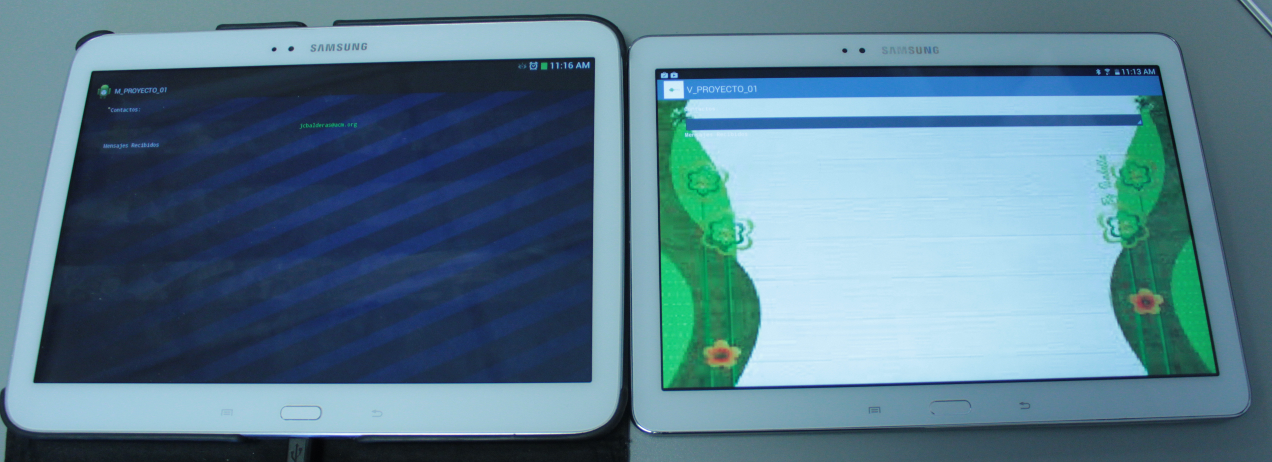
\includegraphics[scale=0.23]{Plagio/Pirata01}
\end{center}
\end{frame}


\begin{frame}
\frametitle{Plagio}
\begin{columns}[c] % The "c" option specifies centered vertical alignment while the "t" option is used for top vertical alignment
\column{.68\textwidth} % Left column and width
\begin{itemize}
\item Reprobación automática a quien copie códigos de Internet y los reporte como suyos, ademas de una nota en su expediente con copia para el consejo de calidad 
\end{itemize}
\column{.28\textwidth} % Left column and width
\begin{center}

\includegraphics[scale=0.27]{Plagio/tarjeta-roja.jpg}
\end{center}
\end{columns}
\begin{center}
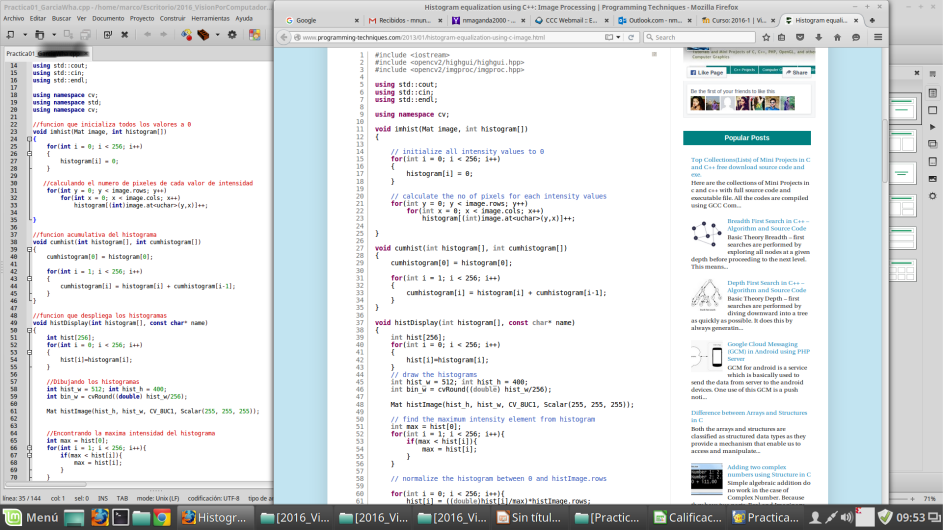
\includegraphics[scale=0.23]{Plagio/Pifia}
\end{center}
\end{frame}

\begin{frame}
\frametitle{Plagio}
\begin{columns}[c] % The "c" option specifies centered vertical alignment while the "t" option is used for top vertical alignment
\column{.68\textwidth} % Left column and width
\begin{itemize}
\item Reprobación automática a quien copie códigos de Internet y los reporte como suyos, ademas de una nota en su expediente con copia para el consejo de calidad 
\end{itemize}
\column{.28\textwidth} % Left column and width
\begin{center}

\includegraphics[scale=0.27]{Plagio/tarjeta-roja.jpg}
\end{center}
\end{columns}
%\url{https://github.com/naman14/AlgorithmVisualizer-Android}
\href{https://github.com/naman14/AlgorithmVisualizer-Android}{https://github.com/naman14/AlgorithmVisualizer-Android}

\begin{columns}[c] % The "c" option specifies centered vertical alignment while the "t" option is used for top vertical alignment
\column{.44\textwidth} % Left column and width
\begin{center}
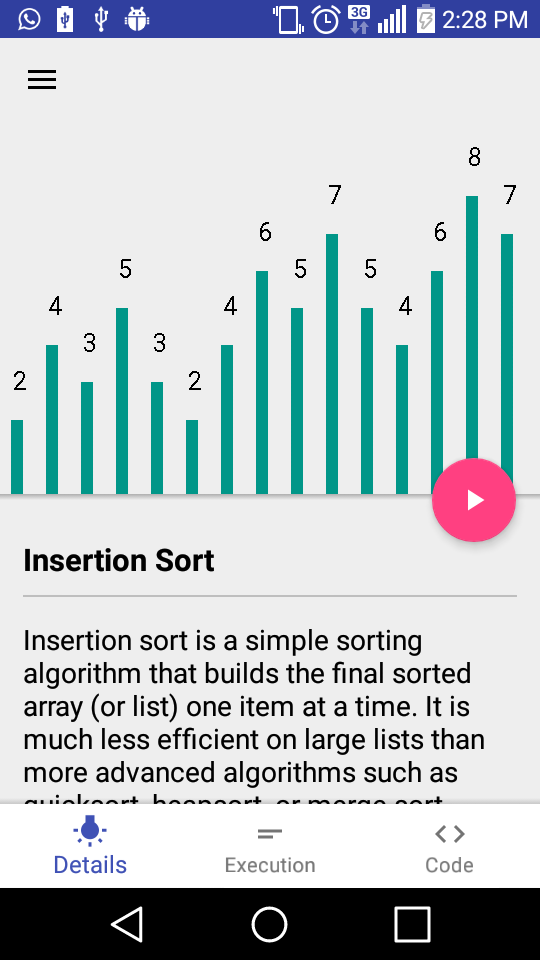
\includegraphics[width=2.3cm]{Plagio/Piratazo_Orig1}\hspace{0.05cm}
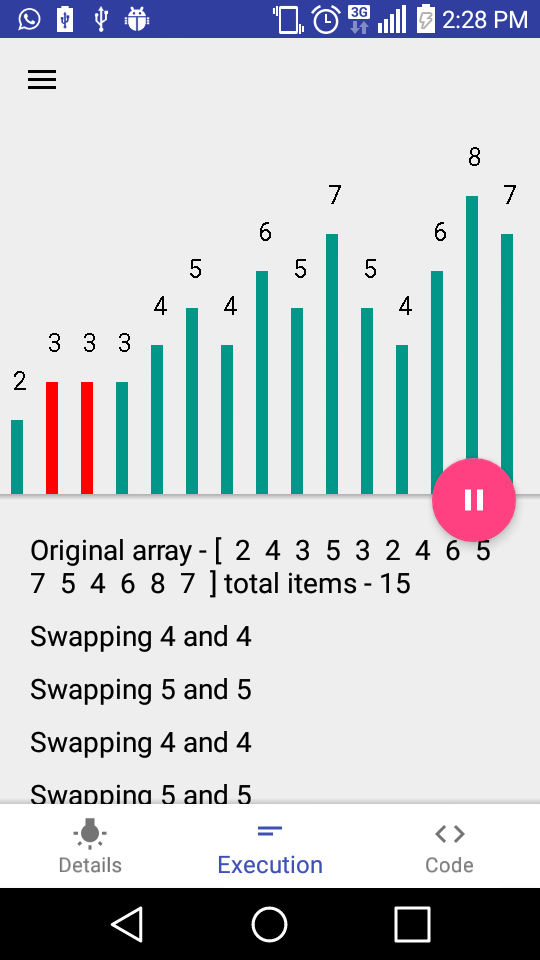
\includegraphics[width=2.3cm]{Plagio/Piratazo_Orig2}\\
Proyecto Original
\end{center}
\column{.44\textwidth} % Left column and width
\begin{center}
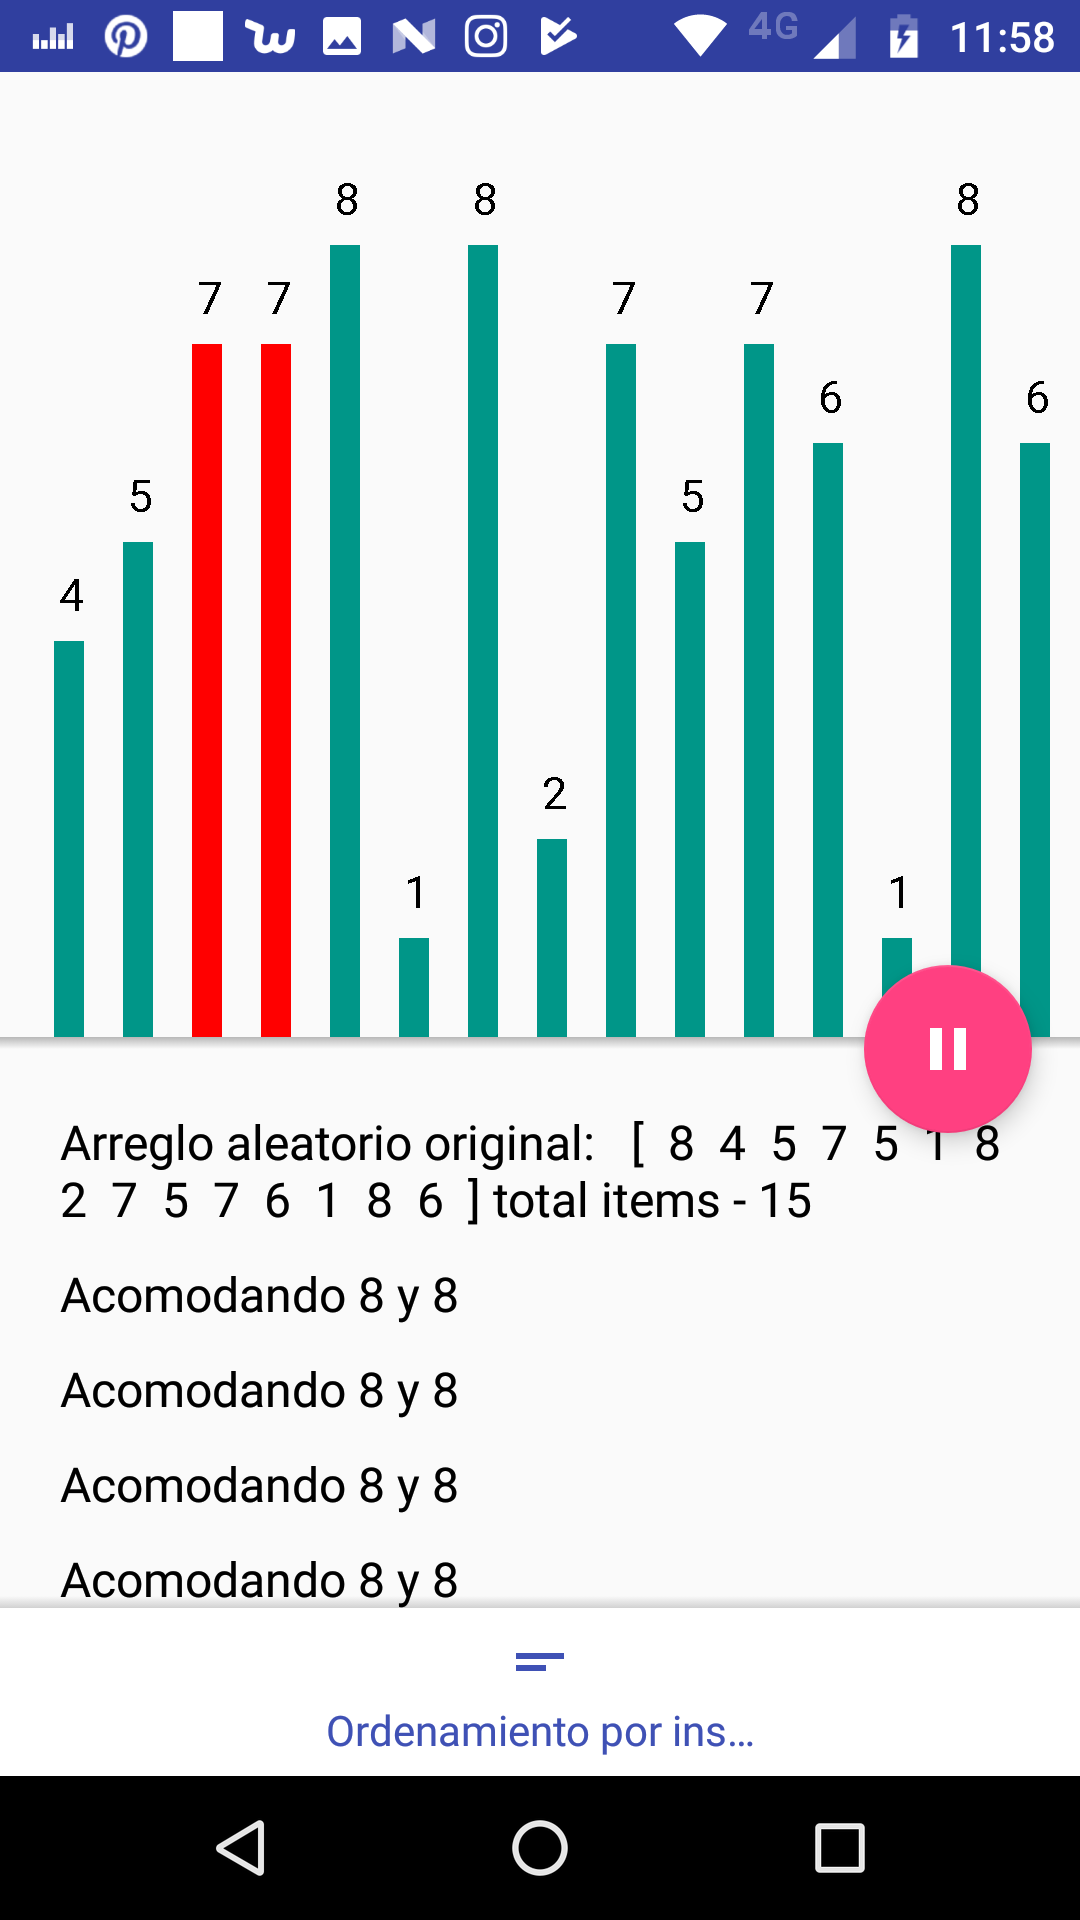
\includegraphics[width=2.3cm]{Plagio/Piratazo_Oscar1}\hspace{0.05cm}
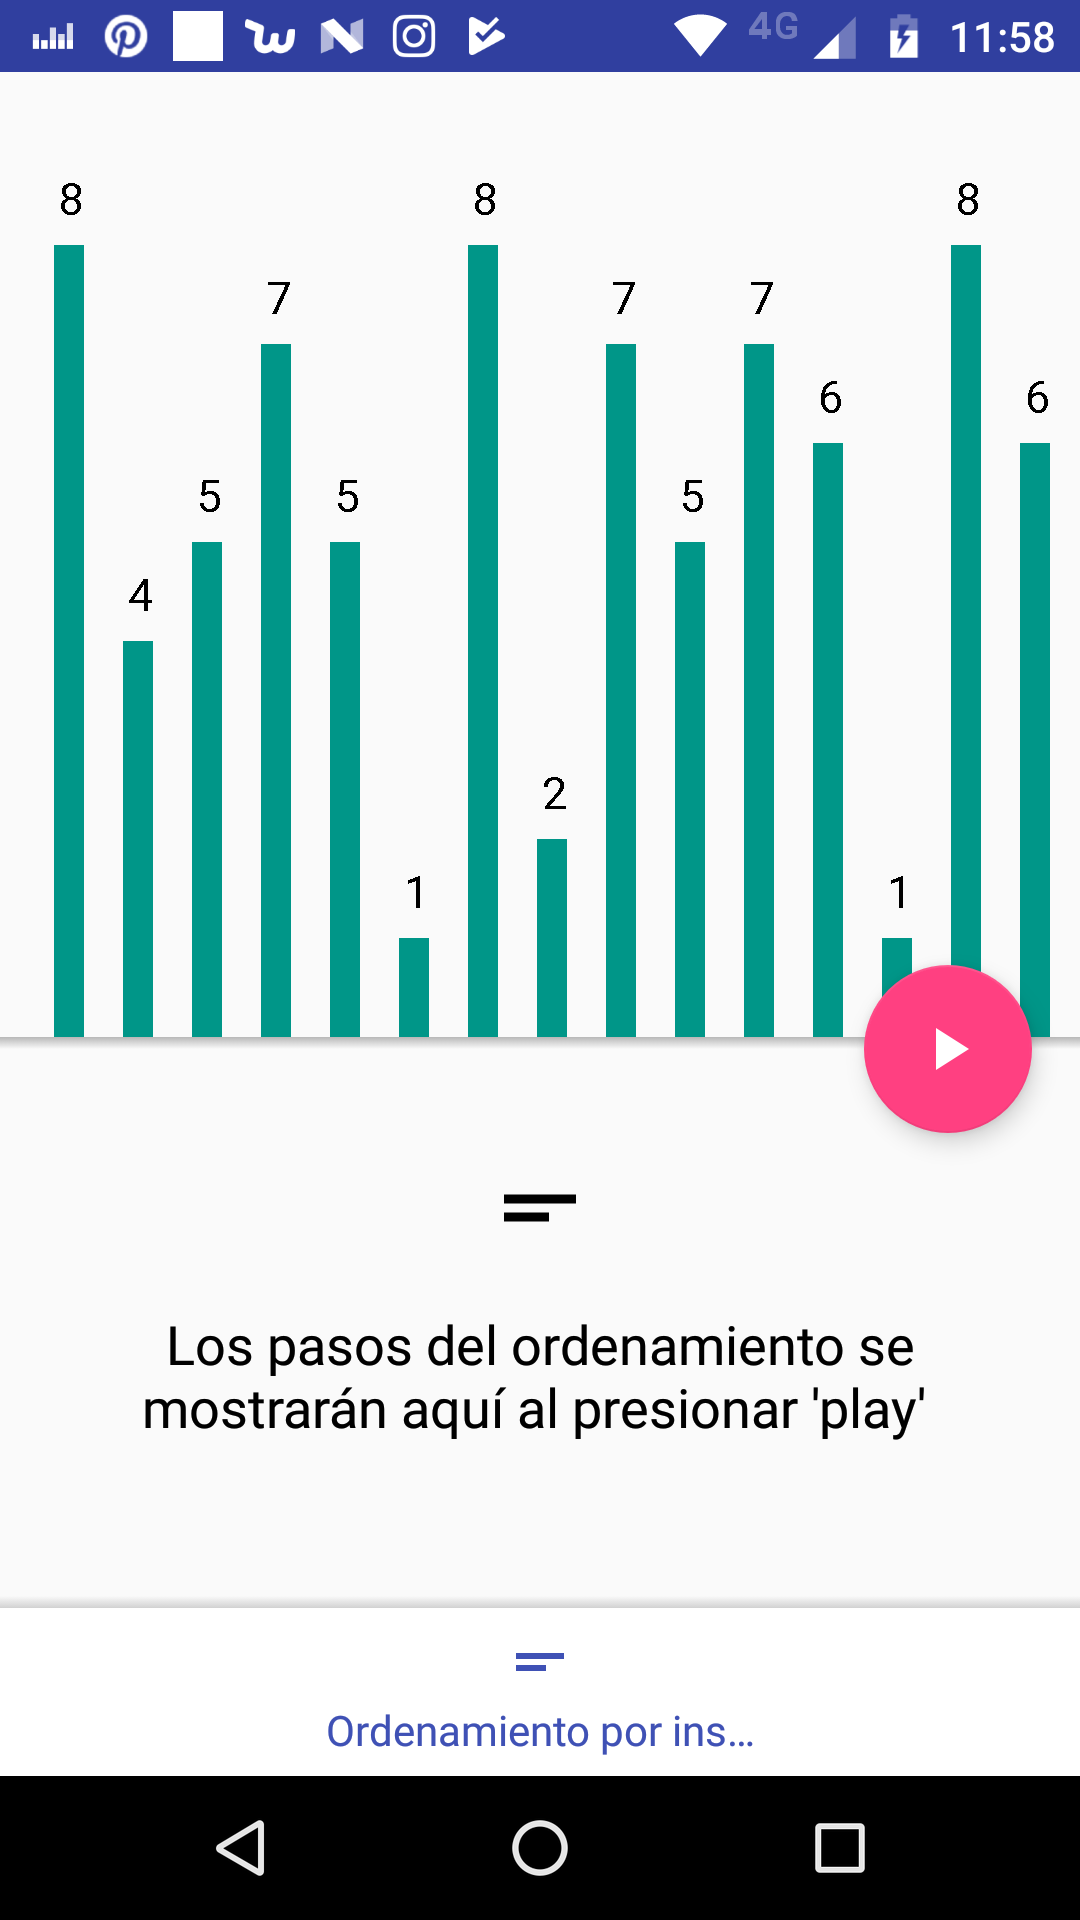
\includegraphics[width=2.3cm]{Plagio/Piratazo_Oscar2}\\
Proyecto ``clonado''
\end{center}	
\end{columns}
\end{frame}





\begin{frame}
\frametitle{Frase célebre}
``Finalmente son jóvenes que están en la preparatoria y que deben de leer su convocatoria con toda claridad, si no cumplen con los requisitos, si no pueden leer una convocatoria que dice tienes que traer número uno esto, número dos esto, número tres esto, no están listos para ser \textbf{estudiantes de educación superior}, así lo digo con toda claridad''.

Sara Ladrón de Guevara.

Rectora de la Universidad Veracruzana (2013-2017 y 2017-2021).

\end{frame}





\begin{frame}
\frametitle{CONCLUSIÓN}
\begin{center}

\includegraphics[scale=0.31]{Conclusion/UNO}
\end{center}
\end{frame}




\end{document}



